\documentclass{article}
\usepackage{graphicx} % Required for inserting images

\title{Atividade de Pesquisa - Macabéa}
\author{Francisco Dall' Oglio Scorsato}
\date{Abril 2024}

\begin{document}

\maketitle
\section{O que é Flor de Mulungu?}
\hspace{\parindent}Flor de Mulungu é uma planta medicinal encontrada no Brasil. Serve para tratar ansiedade, combater insônia e regular a pressão arterial, entre outros benefícios. Tem folhas vermelhas.
\begin{figure}[h]
    \centering
    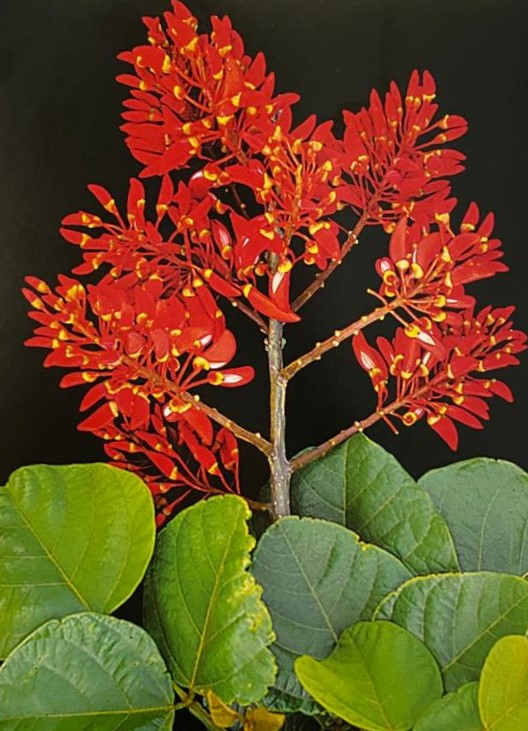
\includegraphics[width=0.5\linewidth]{image_2024-04-08_225403532.png}
\end{figure}
\section{De onde foi tirada a epígrafe do conto?}
\hspace{\parindent}Foi tirada de um livro de Clarice Linspector denominado de "A Hora da Estrela".
\par Clarice Linspector foi uma das mais influentes escritoras brasileiras, e uma das principais figuras da literatura nacional. Sua escrita é conhecida por ser introspectiva e filosófica. 
\par A Hora da Estrela foi o último romance que ela publicou antes de sua morte. Fala sobre uma mulher chamada Macabéa que sai do Nordeste e vai ao Rio de Janeiro buscar uma vida melhor. 

\section{Quem foi Flaubert e Emma Bovary?}
\hspace{\parindent}Gustave Flaubert foi um escritor francês que enlouqueceu. Seu amor impossível por uma mulher casada inspirou diversos livros seus. 
\par Sua primeira obra foi "Madame Bovary", que o levou 5 anos para escrever. Teve uma fala famosa "Emma Bovary c'est moi!"  (Emma Bovary sou eu), para se defender de acusações.

\section{Quem é Agatha Christie? E qual é o caso dos dez negrinhos?}
\hspace{\parindent}Agatha Christie foi uma das maiores escritoras de histórias de mistério, tendo escrito mais que 100. Um de seus livros mais aclamados é "O Caso dos Dez Negrinhos" (renomeado para E Não Sobrou Nenhum". Na história, há um poema que descreve a morte de dez soldados, que vão, um a um, morrendo. Em uma casa, onde dez pessoas se encontram sobre convites misteriosos, morre um por um a cada dia, morrendo de maneiras assustadoramente similares ao poema.
\par Eu não entendi a referência no texto.

\section{Quem é Bráulio Tavares e qual sua relação com os dez negrinhos?}
\hspace{\parindent}Bráulio Tavares é um escritor e poeta brasileiro. Escreveu um poema, paródia daquele no trama de Agatha Christie, porém, com outra mensagem mais crítica, onde dez "negrinhos" morrem, um a um. No final do poema, eles são multiplicados em um milhão.

\section{Quem é Eulália de Marcos Bagno?}
\hspace{\parindent}A Língua de Eulália, um livro de Marcos Bagno, tenta demonstrar que o uso de uma linguagem "diferente" nem sempre pode ser considerado um erro de português. Marcos defende que a diversidade linguística é algo positivo e natural, que deve ser preservado. 

\section{O que você entendeu do conto?}
\hspace{\parindent}O texto parece contar a história da mesma Macabéa de Clarice Linspector. Fala sobre sua vida antes de ir ao Rio de Janeiro e como as pessoas a percebiam. Eu tive a impressão de que a personagem Macabéa era, mesmo dentro do conto, uma personagem. 
\par Depois, é contado o tempo dela na "capital" como datilógrafa, e como era aparentemente infeliz com isso.
\par É referenciada a nacionalidade dela: Portuguesa, Africana e Indígena, todos se juntando para criar o Brasileiro. 
\par No final, parece que ela morre, mas isso causa o nascimento de algo.

\end{document}
